\documentclass[compress]{beamer}
\usetheme{sthlm}

\usepackage{
booktabs,
datetime,
dtklogos,
graphicx,
multicol,
pgfplots,
ragged2e,
tabularx,
tikz,
wasysym
}

\pgfplotsset{compat=1.8}

\usepackage[utf8]{inputenc}
\usepackage[T1]{fontenc}
\usepackage{newpxtext,newpxmath}

\usepackage{listings}
\lstset{ %
language=[LaTeX]TeX,
basicstyle=\normalsize\ttfamily,
keywordstyle=,
numbers=left,
numberstyle=\tiny\ttfamily,
stepnumber=1,
showspaces=false,
showstringspaces=false,
showtabs=false,
breaklines=true,
frame=tb,
framerule=0.5pt,
tabsize=4,
framexleftmargin=0.5em,
framexrightmargin=0.5em,
xleftmargin=0.5em,
xrightmargin=0.5em
}

\usetikzlibrary{
backgrounds,
mindmap
}

\setbeameroption{show notes}

\title{CTF}
\subtitle{Siber güvenlik bilmeceleri}
\date{07.03.2015}
\author{\texttt{Halit Alptekin}}
\institute{BILMOK}

\hypersetup{
pdfauthor = {Halit Alptekin: info@halitalptekin.com},      
pdfsubject = {Cyber Security, },
pdfkeywords = {ctf, cyber security, hacking},  
pdfmoddate= {D:\pdfdate},          
pdfcreator = {LaTeX}
}

\begin{document}

\maketitle

\section*{whoami}
\begin{frame}{whoami}

\begin{itemize}
	\item Bilgisayar mühendisliği öğrencisi
	\item Özgür yazılım ve açık kaynak tutkunu
    \item Siber güvenlik meraklısı
    \item TMD, LKD, Octosec üyesi
    \item Amator telsizci, amatör matematikçi
\end{itemize}

\end{frame}

\section*{Plan}
\begin{frame}{Plan}
\tableofcontents[hideallsubsections]
\end{frame}


\section{CTF}

\begin{frame}{nedir?}

\begin{itemize}
	\item Eğitici ve uygulamalı oyunların genel adıdır
	\item Eski Roma yıllarından beri gerçekleştirilir
    \item Amaç, saldırı ve savunma bilgilerini uygulamaya dökmektir
    \item İsmi bayrak yakalama olsa da amaç her zaman bir bayrağa sahip olmak değildir
\end{itemize}

\end{frame}

\begin{frame}{niye?}

\begin{itemize}
	\item Katılanların farklı düşünme yeteneklerini geliştirir
    \item Sahip olunan teorik bilgilerin, uygulamasını yapma şansı verir
    \item Yeteneklerin ölçülmesi için bir araçtır
    \item Sıkıcı öğrenme yerine, eğlenceli öğrenmeyi amaçlar
    \item Siber güvenlik alanı uygulamalı bir alandır, kitaplarda kalamaz
\end{itemize}

\end{frame}

\begin{frame}{Neler gerekli?}
\centering
\begin{tikzpicture}[scale=0.88]
	\path[mindmap,concept color=sthlmGreen,text=white]
	node[concept] {\textcolor{white}{CTF}}
	[clockwise from=-30]
	child[concept color=sthlmBlue,text=white] { node[concept] {Siber Güvenlik} }
	child[concept color=sthlmLightBlue,text=white] { node[concept] {Programlama} }
	child[concept color=sthlmBlue,text=white] { node[concept] {Zeka} };
\end{tikzpicture}
\end{frame}

\begin{frame}{türleri?}

\begin{itemize}
	\item Jeopardy
	\begin{itemize}
		\item Web
		\item Crypto
        \item Stego
		\item Reverse
        \item Forensic
        \item Binary
        \item Exploit
        \item Programming
        \item Mobile
        \item Misc
	\end{itemize}    
    \item Saldır-savun
	\begin{itemize}
		\item Pentest
	\end{itemize}       
    \item Karışık
\end{itemize}

\end{frame}

\section{Ornekler}

\subsection{Forensic}

\begin{frame}{Forensic 1}
	\begin{figure}
		\centering
		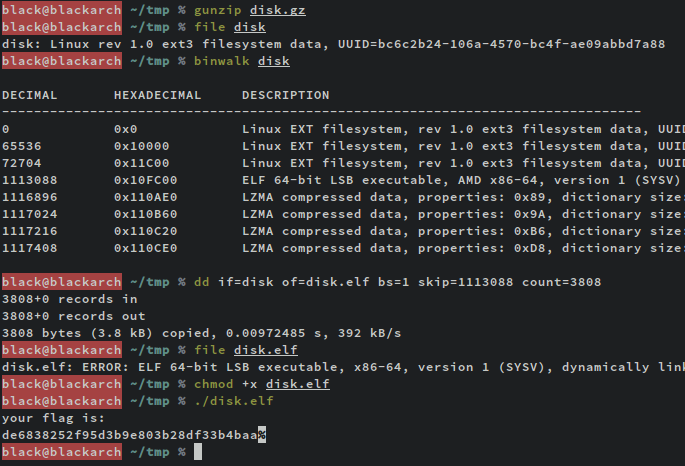
\includegraphics[width=\textwidth]{images/f1.png}
	\end{figure}
\end{frame}

\begin{frame}{Forensic 2}
	\begin{figure}
		\centering
		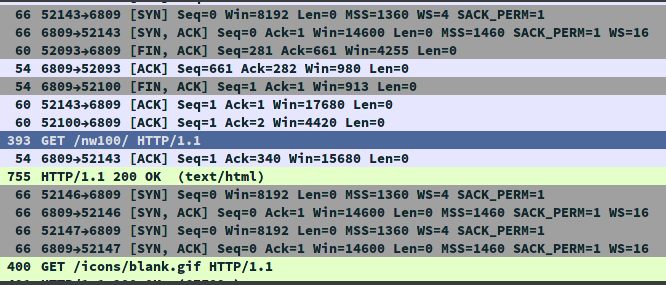
\includegraphics[width=\linewidth]{images/f21.png}
	\end{figure}
\end{frame}

\begin{frame}{Forensic 2}
	\begin{figure}
		\centering
		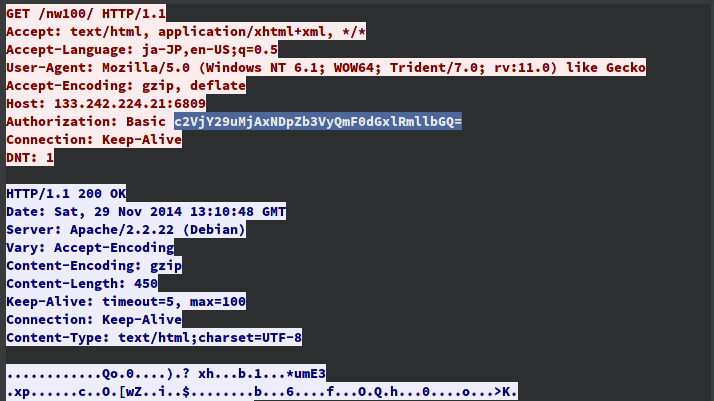
\includegraphics[width=\textwidth]{images/f22.png}
	\end{figure}
\end{frame}

\begin{frame}{Forensic 2}
	\begin{figure}
		\centering
		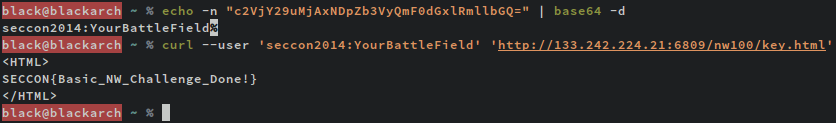
\includegraphics[width=\textwidth]{images/f23.png}
	\end{figure}
	\begin{figure}
		\centering
		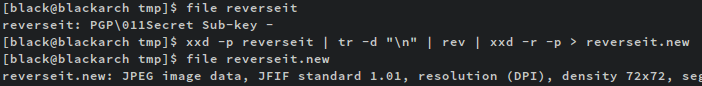
\includegraphics[width=\textwidth]{images/f24.png}
	\end{figure}    
\end{frame}

\subsection{Crypto}

\begin{frame}{Crypto 1}
	\begin{figure}
		\centering
		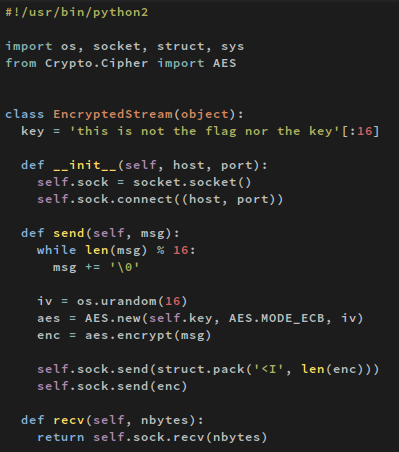
\includegraphics[height=2.8in]{images/c12.png}
	\end{figure}
\end{frame}

\begin{frame}{Crypto 1}
	\begin{figure}
		\centering
		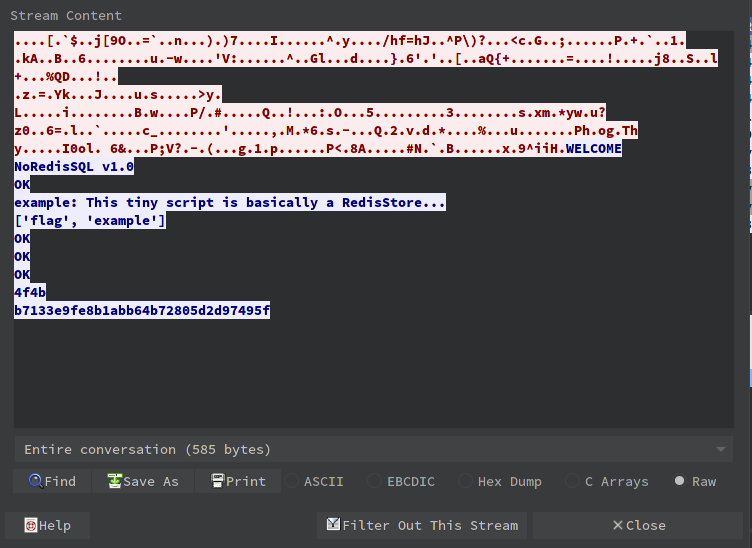
\includegraphics[width=\textwidth]{images/c11.png}
	\end{figure}
\end{frame}

\begin{frame}{Crypto 1}
	\begin{figure}
		\centering
		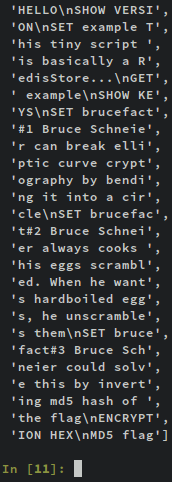
\includegraphics[width=0.2\textwidth,height=1.5in]{images/c13.png}
	\end{figure}
	\begin{figure}
		\centering
		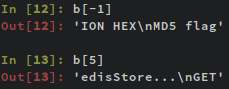
\includegraphics[height=1in]{images/c14.png}
	\end{figure}    
\end{frame}

\subsection{Exploit}

\begin{frame}{Exploit 1}
	\begin{figure}
		\centering
		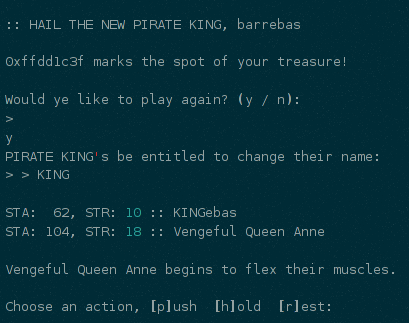
\includegraphics[height=2in]{images/e11.png}
	\end{figure}
	\begin{figure}
		\centering
		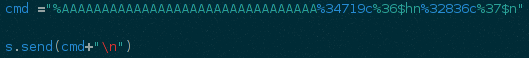
\includegraphics[width=\textwidth,height=0.5in]{images/e12.png}
	\end{figure}    
\end{frame}

\begin{frame}{Exploit 2}
	\begin{figure}
		\centering
		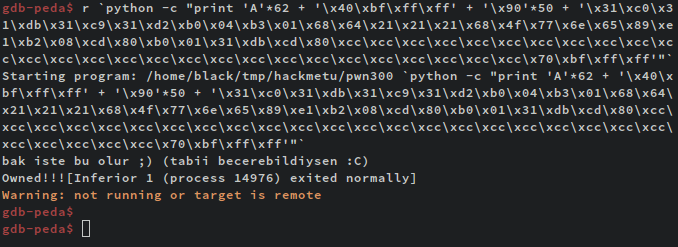
\includegraphics[width=\textwidth]{images/e21.png}
	\end{figure}
\end{frame}

\subsection{Programming}

\begin{frame}{Programming 1}
	\begin{figure}
		\centering
		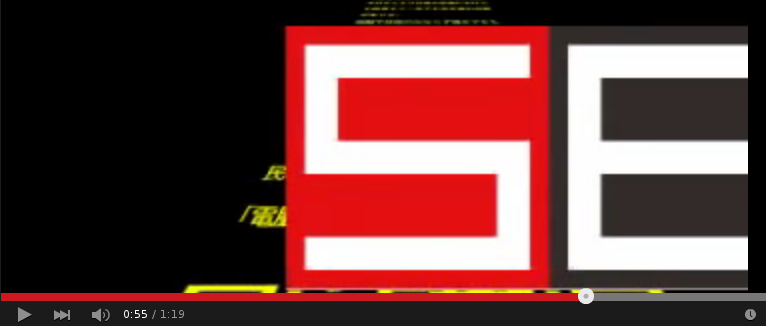
\includegraphics[width=\textwidth]{images/p11.png}
	\end{figure}
\end{frame}

\begin{frame}{Programming 1}
	\begin{figure}
		\centering
		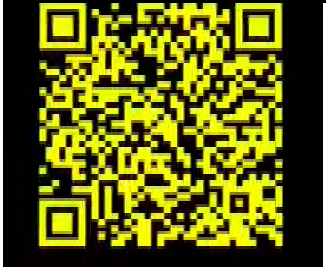
\includegraphics[width=0.8\textwidth]{images/p12.png}
	\end{figure}
\end{frame}

\begin{frame}{Programming 2}
	\begin{figure}
		\centering
		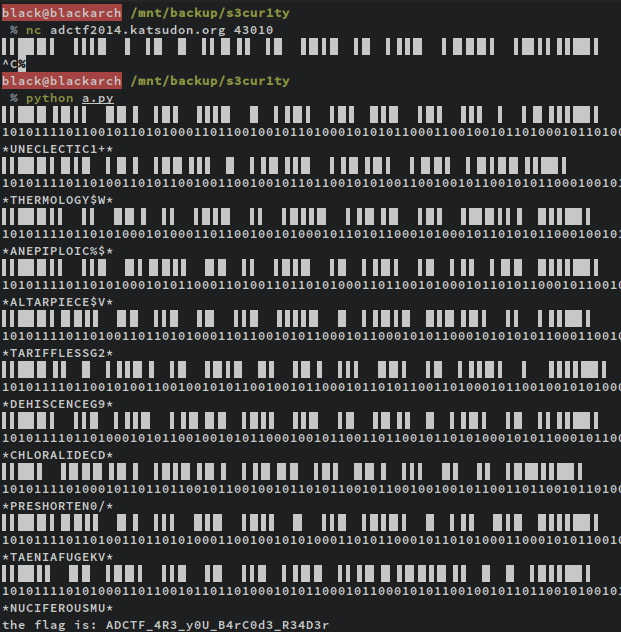
\includegraphics[width=0.8\textwidth,height=3in]{images/p21.png}
	\end{figure}
\end{frame}

\begin{frame}{Programming 3}
	\begin{figure}
		\centering
		
\includegraphics[width=\textwidth]{images/p31.png}
	\end{figure}
\end{frame}

\subsection{Reverse}

\begin{frame}{Reverse 1}
      \begin{figure}
          \centering
          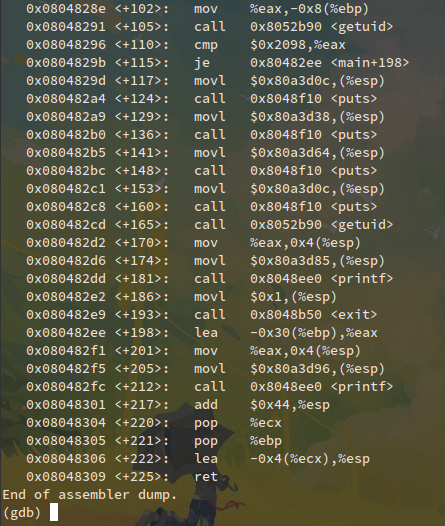
\includegraphics[height=2.8in]{images/r11.png}
      \end{figure}
\end{frame}

\begin{frame}{Reverse 1}
      \begin{figure}
          \centering
          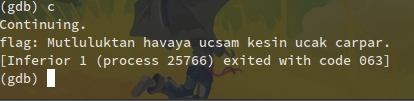
\includegraphics[width=\textwidth]{images/r12.png}
      \end{figure} 
\end{frame}

\begin{frame}{Reverse 2}
	\begin{figure}
		\centering
		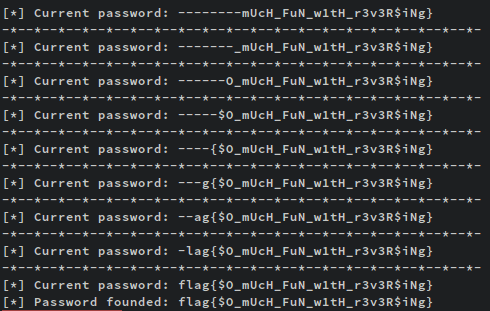
\includegraphics[width=\textwidth]{images/r21.png}
	\end{figure}
\end{frame}

\subsection{Stego}

\begin{frame}{Stego 1}
	\begin{figure}
		\centering
		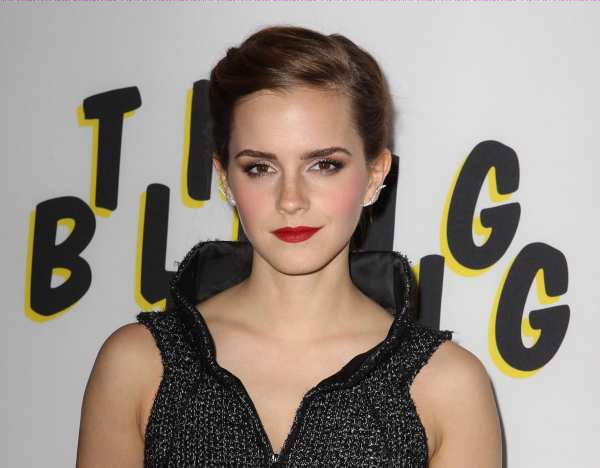
\includegraphics[width=\textwidth,height=2.5in]{images/s11.png}
	\end{figure}
\end{frame}

\subsection{Web}

\begin{frame}{Web}

\begin{itemize}
	\item NoSql injection
    \item PHP exploit
    \item Python micro web frameworks
    \item Perl-cgi exploit
    \item Shelshock
    \item Hearthbleed
\end{itemize}

\end{frame}

\subsection{Mobil}

\begin{frame}{Mobil}

\begin{itemize}
	\item APK decompile
    \item IOS forensic
    \item Android kernel exploitation
\end{itemize}

\end{frame}

\section{Etkinlikler}

\begin{frame}{Türkiye?}

\subsection{Türkiye}

\begin{itemize}
	\item Sibermeydan
    \item Hackmetu
    \item Kızımız Pek Hacker
    \item Hack2Net
    \item Dünyayı Kurtaran Hacker
\end{itemize}

\end{frame}

\subsection{Yurtdışı}

\begin{frame}{Yurtdışı?}

\begin{itemize}
	\item Ghost in the Shellcode
    \item RuCTF
    \item PlaidCTF
    \item 9447
    \item Seccon
    \item Boston Key Party CTF
    \item HackIM
\end{itemize}

\end{frame}

\subsection{Wargames}

\begin{frame}{Hazırlık?}

\begin{itemize}
	\item http://www.smashthestack.org/
    \item http://www.overthewire.org/wargames/
    \item http://www.hackthissite.org/
    \item http://exploit-exercises.com/
    \item http://vulnhub.com/
    \item http://computer-forensics.sans.org/community/challenges
    \item http://hax.tor.hu/
    \item https://pwn0.com/
    \item http://www.damnvulnerablelinux.org/
    \item http://www.ethicalhack3r.co.uk/damn-vulnerable-web-app/
    \end{itemize}
\end{frame}

\section{Referans}

\subsection{Diğerleri}

\begin{frame}{Geri Kalanlar}

\begin{itemize}
	\item http://www.smashthestack.org/
	\item http://trailofbits.github.io/ctf/
	\item http://captf.com/practice-ctf/
	\item http://captf.com/
	\item http://ftp.hackerdom.ru/ctf-images/
	\item http://shell-storm.org/repo/CTF/
	\item https://ctftime.org
	\item http://clist.by/
    \end{itemize}
\end{frame}

\begin{frame}{Son}
	Sunumu kaynak kodları ile beraber Github adresimde bulabilirsiniz.
	\begin{itemize}
    	\item \url{github.com/halitalptekin}
        \item \url{twitter.com/halitalptekin}
		\item \url{info@halitalptekin.com}
	\end{itemize}
\end{frame}

\end{document}